\documentclass[a4paper, 12pt, notitlepage]{report}

\usepackage{amsfonts} % if you want blackboard bold symbols e.g. for real numbers
\usepackage{graphicx} % if you want to include jpeg or pdf pictures
\usepackage{geometry}
\usepackage{subfigure}
\geometry{verbose,a4paper,tmargin=30mm,bmargin=30mm,lmargin=30mm,rmargin=30mm}


\begin{document}

%%%%%%%%%% PRELIMINARY MATERIAL %%%%%%%%%%
\begin{titlepage}
\newcommand{\horrule}[1]{\rule{\linewidth}{#1}} 	% Horizontal rule
\begin{center}
		\usefont{OT1}{bch}{b}{n}
		\horrule{0.5pt} \\
		\usefont{OT1}{bch}{b}{n}
		\huge BIOMORPHIC PALM USING ARDUINO \\
		\horrule{2pt} \\
		\end{center}
		{\centering
		\vspace{1cm}
		\\minip/ece@nssce/1014/23.28\\
		\vspace{1cm}
\large\bf{\emph{MINI PROJECT REPORT}}\\

\it{As a partial fulfilment of the curriculum}\\
\vspace{0.25cm}
\vspace{0.1cm}
\vspace{1cm}
\it
by \\
\vspace{0.5cm}
\rm
{\large \bf {\emph{RAHUL R NAIR (NSAKEEC066)\\ SREERAG S (NSAKEEC086)\\VISHNU K (NSAKEEC097)\\VISHNU S DEV (NSAKEEC099)}}}\\

\vspace{1.0cm}

{\it{under the guidance of}} \\
\vspace{0.5cm}
\hspace{0.05cm} {\large \bf {Mrs. ASHA T S}}\\
\hspace{0.025cm} {\large \bf {Associate Professor}}\\
\vspace {0.5cm}
\vspace {0.5cm}
\begin{figure}[h]
{\centering {\includegraphics[scale=0.8]{logo.png}}\par}
\end{figure}
\begin{center}
Department of Electronics \& Communication Engineering \\
NSS College OF Engineering, Palakkad \\March 2013
\end{center}
}
\end{titlepage}

\newpage
\section*{
\begin{center}
NSS College OF Engineering, Palakkad  \\
\end{center}}

\begin{figure}[h!]
{\centering {\includegraphics[scale=0.85]{logo.png}}\par}
\end{figure}

\begin{center}
\textbf{Department of Electronics \& Communication Engineering}  \\
\end{center}}

\section*{
\begin{center}
CERTIFICATE \\
\end{center}}\\

\subsubsection{\vspace{0.25cm}Certified that mini project work titled BIOMORPHIC PALM USING \vspace{0.25cm} ARDUINO is a bonafied work carried out in sixth semester by Rahul R \vspace{0.25cm}Nair, Sreerag S, Vishnu K and Vishnu S Dev during the academic year \vspace{0.25cm} of 2012-2013 under the guidance of the department as part of the partial \vspace{0.25cm} fulfillment for the award of Bachelor of Technology in ELECTRONICS \vspace{0.25cm} AND COMMUNICATION ENGINEERING from University of Calicut \vspace{0.25cm} and no part of this work has been submitted earlier for the award of any degree.}\\
\vspace{3.0cm}
\textbf{PROJECT GUIDE} \hspace{5.0cm} \textbf{HEAD OF DEPARTMENT}\\
\vspace{0.25cm}
Mrs.Asha.T.S \hspace{6.3cm} Mr.ABDUL KAREEM
\newpage
\section*{\begin{center}{ACKNOWLEDGEMENT}\end{center}} % this must be included in undergradate projects
\vspace{1.0in}
We express our sincere piece of gratitude to Mr.Abdul Kareem ,Head Of Electronics And Communication Department for his moral support and encouragement\\

We would like to express our deep sense of gratitude to our project guide Prof.Asha T S, Department of Electronics and Communication, for being a great force behind all our efforts through her advice, guidance, and encouraging nature. \\

We acknowledge the help of Prof. Vinod G for his guidance and motivation throughout the project.\\
 
Finally we would like express our gratitude towards our parents for their moral and financial support for making this project a success\\

\vspace{5.0cm}
\begin{flushright}
{RAHUL R NAIR (NSAKEEC066)\\ SREERAG S (NSAKEEC086)\\VISHNU K (NSAKEEC097)\\VISHNU S DEV (NSAKEEC099)\\
\end{flushright}
\vspace{1.0cm}
March 2013\\
Department of Electronics \& Communication Engineering\\
NSS College Of Engineering,Palakkad
\newpage

\newpage
\section*{\begin{center}{ABSTRACT}\end{center}}
\\

The developing technology of the future, biomorphic robotics, strictly limited inside ethical dimensions, aids the humans for accomplishing tedious tasks which can’t be done by them due to physical limitations. Biomorphic robotics is a sub discipline of robotics focused on the emulating mechanics, sensing, structural, and computing systems of animals. They deal with how biologically inspired principles can be used to negotiate complexities of real world.\\

 			By this project we are trying to engineer a robotic palm which can mimic the actions of a human palm using a biomorphic system .Retaining human control over machines is the most important aspect of robotics. Hence we are planning to adopt a wireless system for the transmission and reception of the instantaneous positions of human palm. Using a combination of servomotors, and pulleys the robotic palm can be equipped with ability to move as the human palm does.\\
			
Form the electronics side of view we are using Arduino, a powerful open source electronic prototyping platform to realize this system. For programming the machine we are using Arduino IDE a cross-platform application written in Java.
By the end of project we are trying to accomplish the following \\

\begin{enumerate}
\item To explore the possibilities of robotics in simplifying complex tasks were our imagination is the only limit.
\item Demonstrate the power of Arduino platform to realize complex    electronic systems with ease and simplicity
\item To develop a plan of action for improving the current developed system   into a complex humanoid robot possibly as a part of main project in coming semesters.
 \end{enumerate}

\tableofcontents
\listoffigures 

%%%%%%%%%% MAIN TEXT STARTS HERE %%%%%%%%%%

%%%%%%%%%% SAMPLE CHAPTER %%%%%%%%%%
\chapter{INTRODUCTION}
\\

Simplicity and high accuracy have become the two contradictory needs of any industrial process. By introducing autonomous robotic applications, tedious tasks can be accomplished keeping the demands of the accuracy and simplicity in mind. However, developing these applications for industries specific to countries like India, where cheap labor is available, becomes a major problem to be tackled in terms of cost.\\

Human control over the developed robotic system is the most significant aspect of robotics. Keeping this in mind an idea of a robotic palm mimicking the actions of a human palm was developed.  A study regarding the possibilities of this idea was conducted first and exciting results were obtained. As a second stage selection of hardware for the implementation was done giving priority to low cost and simplicity. Thus Arduino platform satisfying both the needs stated above was selected. This project is a practical application of the basic principles of electronics and wireless communication.\\

The biomorphic palm system consists of flex sensing system , a Micro controller for processing the sensor inputs , a radio frequency transmitter- receiver pair , servo motors and power transfer cords and a mechanical palm made of plastic tubes. The system presented here is a prototype and can be developed much more for better performance and efficiency. \\ 

\newpage
\chapter{PROJECT OVERVIEW}
\\
Even though the idea and principle behind this biomorphic system is simple, like in every engineering structures here also precise measurements, accurate and flawless planning and design are needed. The working of the system is so simple that even a layman can understand.\\
The system is divided to two main modules\\

\begin{enumerate}
\item POWER GLOVES
\item BIOMORPHIC PALM

\end{enumerate}

	The power gloves are attached with the 5 flex sensors which are capable of chemically varying their resistance, with respect to the angle they are flexed to. A circuit is designed for converting this variation in resistance to corresponding voltage equivalent. So basically the power gloves act as a resistance to voltage converter. This analog voltage is given to the Arduino embedded system as an input to the atmega 328 microcontroller through the analog input pin provided in the board. The coding algorithm on the processor maps these values to a range of 0 to 256 and is radiated to space using the xbee (2mw) transmitter chip onboard.\\

	The biomorphic palm is attached with another Arduino system with a receiving xbee chip paired with the transmitter onboard the gloves. The receiver receives the signal and is fed to the processor. Using decoding algorithm the mapped values are converted to the original values and is made available at the output pins from which they are applied on to the servo motors. The servo motors responds to the voltage and the movements of the motor is transferred to the palm using power transfer cords attached to the motors.\\

\begin{figure}[h!]
{\centering {\includegraphics[scale=0.5]{fig1.png}}}
\caption{POWER GLOVES}
\end{figure}
 
\newpage   
\section{ARDUINO}
%
Arduino is an open-source electronics prototyping platform based on flexible, easy-to-use hardware and software. It's intended for artists, designers, hobbyists, and anyone interested in creating interactive objects or environments. It is a single-board microcontroller designed to make the process of using electronics in multidisciplinary projects more accessible. The hardware consists of a simple open source hardware board designed around an 8-bit Atmel AVR microcontroller, though a new model has been designed around a 32-bit Atmel ARM. The software consists of a standard programming language compiler and a boot loader that executes on the microcontroller.\\

\begin{figure}[h!]
{\centering {\includegraphics[scale=1]{fig2.png}}\par}
\caption{Arduino Logo} \\
\end{figure}

Arduino boards can be purchased pre-assembled or do-it-yourself kits. Hardware design information is available for those who would like to assemble an Arduino by hand. There are sixteen official Arduinos that have been commercially produced to date. Numerous hardware variations of the Arduino are being sold by third parties.\\

\subsection{Hardware}

An Arduino board consists of an Atmel 8-bit AVR microcontroller with complementary components to facilitate programming and incorporation into other circuits. An important aspect of the Arduino is the standard way that connectors are exposed, allowing the CPU board to be connected to a variety of interchangeable add-on modules known as shields. Some shields communicate with the Arduino board directly over various pins, but many shields are individually addressable via an I²C serial bus, allowing many shields to be stacked and used in parallel. Official Arduinos have used the mega AVR series of chips, specifically the ATmega8, ATmega168, ATmega328, ATmega1280, and ATmega2560. A handful of other processors have been used by Arduino compatibles. Most boards include a 5 volt linear regulator and a 16 MHz crystal oscillator (or ceramic resonator in some variants), although some designs such as the LilyPad run at 8 MHz and dispense with the on board voltage regulator due to specific form-factor restrictions. An Arduino's microcontroller is also pre-programmed with a boot loader that simplifies uploading of programs to the on-chip flash memory, compared with other devices that typically need an external programmer. \\

\begin{figure}[h!]
{\centering {\includegraphics[scale=1]{Breakoutboard.png}}\par}
\caption{Breakout Board for Arduino-XBEE Interfacing} \\
\end{figure}
 

At a conceptual level, when using the Arduino software stack, all boards are programmed over an RS-232 serial connection, but the way this is implemented varies by hardware version. Serial Arduino boards contain a simple inverter circuit to convert between RS-232-level and TTL-level signals. Current Arduino boards are programmed via USB, implemented using USB-to-serial adapter chips such as the FTDI FT232. Some variants, such as the Arduino Mini and the unofficial Boarduino, use a detachable USB-to-serial adapter board or cable, Bluetooth or other methods. (When used with traditional microcontroller tools instead of the Arduino IDE, standard AVR ISP programming is used.)\\

The Arduino board exposes most of the microcontroller's I/O pins for use by other circuits. The Diecimila, Duemilanove, and current Uno provide 14 digital I/O pins, six of which can produce pulse-width modulated signals, and six analog inputs. These pins are on the top of the board, via female 0.1 inch headers. Several plug-in application shields are also commercially available.\\

The Arduino Nano, and Arduino-compatible Bare Bones Board and Boarduino boards may provide male header pins on the underside of the board to be plugged into solderless breadboards.\\

\begin{figure}[h!]
{\centering {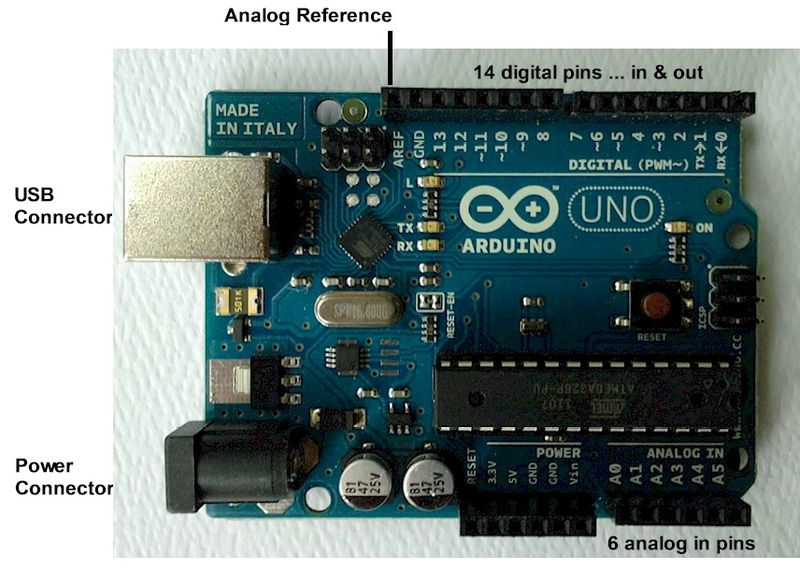
\includegraphics[scale=0.65]{fig3.png}}}
\caption{Arduino UNO Board}
\end{figure}

There are a great many Arduino-compatible and Arduino-derived boards. Some are functionally equivalent to an Arduino and may be used interchangeably. Many are the basic Arduino with the addition of commonplace output drivers, often for use in school-level education to simplify the construction of buggies and small robots. Others are electrically equivalent but change the form factor, sometimes permitting the continued use of Shields, sometimes not. Some variants even use completely different processors, with varying levels of compatibility.\\

\subsection{Software}

The Arduino integrated development environment (IDE) is a cross-platform application written in Java, and is derived from the IDE for the language and the Wiring projects. It is designed to introduce programming to artists and other newcomers unfamiliar with software development. It includes a code editor with features such as syntax highlighting, brace matching, and automatic indentation, and is also capable of compiling and uploading programs to the board with a single click. There is typically no need to edit make files or run programs on a command-line interface.\\

Arduino programs are written in C or C++. The Arduino IDE comes with a software library called "Wiring" from the original Wiring project, which makes many common input/output operations much easier. Users only need define two functions to make a runnable cyclic executive program: \\

\begin{figure}[h!]
{\centering {\includegraphics[scale=0.65]{fig4.png}}\par}
\caption{Arduino 1.0.1 IDE}
\end{figure}

\begin{itemize}
\item Setup() :  a function run once at the start of a program that can initialize settings
\item Loop() : a function called repeatedly until the board powers off

\end{itemize}


The Arduino IDE uses the GNU tool chain and AVR Libc to compile programs, and uses avrdude to upload programs to the board.
As the Arduino platform uses Atmel microcontrollers, Atmel's development environment, AVR Studio or the newer Atmel Studio,  may also be used to develop software for the Arduino.\\ 

\subsection{Development}

The core Arduino developer team is composed of Massimo Banzi, David Cuartielles, Tom Igoe, Gianluca Martino, David Mellis and Nicholas Zambetti. Massimo Banzi was interviewed on the March 21st, 2009 episode (Episode 61) of FLOSS Weekly on theTWiT.tv network, in which he discussed the history and goals of the Arduino project.[16]He also gave a talk at TEDGlobal 2012 Conference, where he outlined various uses of Arduino boards around the world. \\

Arduino is open source hardware: the Arduino hardware reference designs are distributed under a Creative Commons Attribution Share-Alike 2.5 license and are available on the Arduino Web site. Layout and production files for some versions of the Arduino hardware are also available. The source code for the IDE and the on-board library are available and released under the GNU General Public License, version 2. \\

Although the hardware and software designs are freely available under copy left licenses, the developers have requested that the name "Arduino" be product and not be used for derivative works without permission. The official policy document on the use of the Arduino name emphasizes that the project is open to incorporating work by others into the official product. Several Arduino-compatible products commercially released have avoided the "Arduino" name by using "-duino" name variants.\\ 


\chapter{SYSTEM DESIGN}

Flawless Design is the inevitable property for any system to produce desired and expected result. Humans can move just by a thought without thinking about any steps of action. But for mobilizing a robot precise instructions and directions should be given to the system. For this a flawless design process is required\\

\section{DESIGN}

A modular approach always simplifies the design of any system .Hence this project was divided in to modules and each module were individually constructed and was assembled at the final stage. The Biomorphic palm system dealt in this project can be divided in to 4 modules.\\

\begin{enumerate}
\item Sensing Module
\item Coding and Transmission Module
\item Reception and Decoding Module
\item Power Transmission Module 

\end{enumerate}

\newpage
\begin{figure}
{\includegraphics[scale=1.4]{block1.png}}
\caption{Basic System Structure}
\end{figure}

\subsection{Sensing Module}

As the system is designed to mimic the actions of a human palm in it is necessary for the system to have the knowledge of the instantaneous position and state of the human palm. The positions of the 5 fingers were detected using flex sensors. Flex sensors are basically variable resistance. Trough chemical reactions they are able to vary their resistance in response to the bending occurred. \\

Tests were conducted to have the idea about the maximum and minimum resistance values of the sensors in the range of angles at which bending is required.\\

\begin{figure}[h!]
{\centering {\includegraphics[scale=0.75]{fig5-graph.png}}\par}
\caption{Sensor Values}
\end{figure}

\begin{figure}[h!]
{\centering {\includegraphics[scale=0.75]{fig6-stickgraph.png}}\par}
\caption{Fully Extended Sensor Values}
\end{figure}

\begin{figure}[h!]
{\centering {\includegraphics[scale=0.75]{fig7-stickgraph2.png}}\par}
\caption{Sensor Values when fingers at various positions}
\end{figure}

These values are of great importance because; their presence in the coding algorithm improved the accuracy of the total system.\\

\newpage
\newpage
\subsection{Coding And Transmission Module}

The maximum and minimum values of resistance available from the resistance was calculated and tabulated for analysis during the construction of previous module.\\
 
\begin{figure}[h!]
{\centering {\includegraphics[scale=0.75]{fig8.png}}\par}
\caption{Circuit For Sensor Value Range Determination}
\end{figure}

Making use of above circuit and associated code(In coding section) the range of values of resistance and their corresponding voltage converted value for angle at wich the sensor is bend was determined. This value was mapped on to a range of 0 to 255 corresponding to 10 bit adc avialable in the board. This digitzed value was transmitted using xbee 2 chip.\\

\subsection{Reception And Decoding Module}

The Digitized values transmitted by the transmitter were received by the reciever paired with the transmitter.this values were converted back to their original values and was made available at the output ports.\\

\subsection{Power Transmission Module}

Power transmission modules comprise of 5 servo motors and corresponding power transmisson cords. Servo motors of 1.4Nm torque and operating range of 4.8-6 V were used for powering up the biomorphic palm. High tensile plastic wires were used to deliver the motor power to the fingers which were precisely designed using plastic tubes and pipes.\\

\subsection{Circuit Diagrams}
\begin{figure}[h!]
{\centering{\includegraphics[scale=0.4]{flexschem.jpg}}\par}
\caption{Transmitter Side Schematic}
\end{figure}

\begin{figure}[h!]
{\centering{\includegraphics[scale=0.5]{servo2.jpg}}\par}
\caption{Receiver Side Schematic}
\end{figure}

\newpage
\subsection{PCB Layout Design}
\begin{figure}[h!]
{\centering{\includegraphics[scale=1]{handside.png}}\par}
\caption{Transmitter Side layout}
\end{figure}\\

\begin{figure}[h!]
{\centering{\includegraphics[scale=1]{motorside.png}}\par}
\caption{Receiver Side layout}
\end{figure}

The layouts were designed in Eagle CAD and etched out by ourselves

\begin{figure}
\centering
\mbox{\subfigure{\includegraphics[scale=0.08]{DSC_0118.jpg}}\quad
\subfigure{\includegraphics[scale=0.08]{DSC_0143.jpg} }}
\end{figure}

\begin{figure}
\centering
\mbox{\subfigure{\includegraphics[scale=0.08]{DSC_0147.jpg}}\quad
\subfigure{\includegraphics[scale=0.08]{DSC_0148.jpg} }}
\end{figure}

\begin{figure}
\centering
\mbox{\subfigure{\includegraphics[scale=0.08]{DSC_0126.jpg}}\quad
\subfigure{\includegraphics[scale=0.08]{DSC_0128.jpg} }}
\end{figure}

\begin{figure}
\centering
\mbox{\subfigure{\includegraphics[scale=0.08]{DSC_0129.jpg}}\quad
\subfigure{\includegraphics[scale=0.08]{DSC_0170.jpg} }}
\end{figure}

\begin{figure}
\centering
\mbox{\subfigure{\includegraphics[scale=0.08]{DSC_0174.jpg}}\quad
\subfigure{\includegraphics[scale=0.08]{DSC_0177.jpg} }}
\caption{Etching Process} \label{fig12}
\end{figure}

\chapter{TOOLS USED}
\section{FLEX SENSORS}

The flex sensor is a sensor which varies its resistance when they are bend through an angle. As bending angle increases its resistance increases. One side of the sensor is printed with a polymer ink that has conductive particles embedded in it. When the sensor is straight, the particles give the ink a resistance of about 30k Ohms. When the sensor is bent away from the ink, the conductive particles move further apart, increasing this resistance (to about 50k Ohms when the sensor is bent to 90º, as in the diagram below). When the sensor straightens out again, the resistance returns to the original value. By measuring the resistance, you can determine how much the sensor is being bent.\\

\begin{figure}[h!]
{\centering {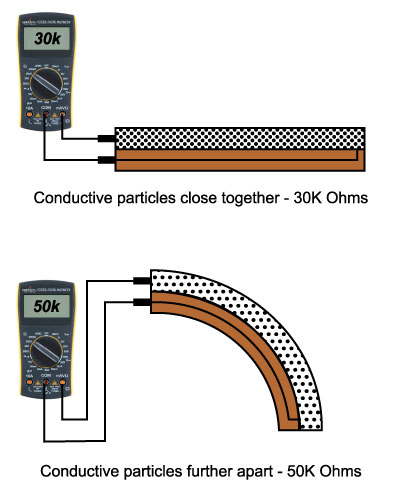
\includegraphics[scale=1]{fig9.png}}\par}
\caption{Sensor Value Determination}
\end{figure}

\newpage
\section{SERVO MOTOR}

Servo refers to an error sensing feedback control which is used to correct the performance of a system. Servo or RC Servo Motors are DC motors equipped with a servo mechanism for  precise  control  of  angular  position.  The  RC  servo  motors  usually  have  a  rotation  limit from 90° to 180°. But servos do not rotate continually. Their rotation is restricted in between the fixed angles. \\

\begin{figure}[h!]
{\centering {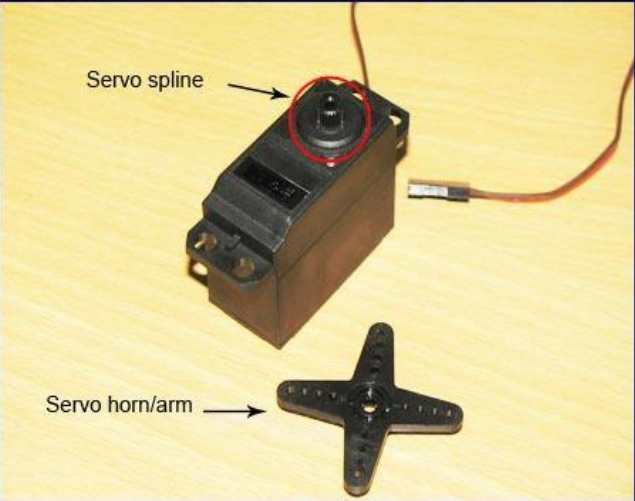
\includegraphics[scale=0.65]{fig10.png}}\par}
\caption{Servo Motor}
\end{figure}

A servo motor mainly consists of a DC motor, gear system, a position sensor which is mostly a potentiometer, and control electronics. The DC motor is connected with a gear mechanism which provides feedback to a position sensor which is mostly a potentiometer. From the gear box, the output of the motor is delivered via servo spline to the servo arm. The potentiometer changes  position  corresponding  to  the  current  position  of  the  motor.  So the  change  in resistance produces an equivalent change in voltage from the potentiometer. A pulse width modulated  signal  is  fed  through  the  control  wire.\\ 

\begin{figure}[h!]
{\centering {\includegraphics[scale=0.85]{servo.jpg}}\par}
\caption{Servo Motor Connecton Diagram}
\end{figure}

 The  pulse  width  is  converted  into  an equivalent  voltage  that  is  compared  with  that  of  signal  from  the  potentiometer  in  an  error amplifier. The servo motor can be moved to a desired angular position by sending PWM (pulse width modulated)  signals  on  the  control  wire. The  servo  understands  the  language  of  pulse position  modulation.  A  pulse  of  width  varying  from  1  millisecond  to  2  milliseconds  in  a repeated time frame is sent to the servo for around 50 times in a second. The width of the
pulse determines the angular position.

\section{XBEE 2s PRO}

XBee is the brand name from Digi International for a family of form factor compatible radio modules. The first XBee radios were introduced under theMaxStream brand in 2005[2] and were based on the 802.15.4-2003 standard designed for point-to-point and point-to-multipoint communications at over-the-air baud rates of 250 kbit/s.[3]\\

Two models were initially introduced—a lower cost 1 mW XBee and the higher power 100 mW XBee-PRO.[4] Since the initial introduction, a number of new XBee radios have been introduced and all XBees are now marketed and sold under the Digi brand. The XBee radios can all be used with the minimum four number of connections – power (3.3 V), ground, data in and data out (UART), with other recommended lines being Reset and Sleep.[5] Additionally, most XBee families have some other flow control, I/O, A/D and indicator lines built in. A version of the XBees called the Programmable XBee has an additional on board processor for user’s code. The Programmable XBee and a new surface mount (SMT) version of the XBee radios were both introduced in 2010\\

\begin{figure}[h!]
{\centering {\includegraphics[scale=0.65]{fig11.png}}\par}
\caption{XBEE Modules}
\end{figure}

\subsection{Form Factors,Antennas And Data Modes}

XBee Modules are available in two form-factors; Through-Hole and Surface Mount. All XBees (with the exception of the XBee 868LP) are available in the popular 20-pin Through-Hole form-factor. Certain XBee modules are also available in a 37-pad Surface Mount design, which is popular for higher volume applications due to the reduced manufacturing costs of SMT technology.\\

XBee Modules typically come with several antenna options, including U.FL, PCB Embedded, Wire, and RPSMA.
The XBees can operate either in a transparent data mode or in a packet-based application programming interface (API) mode. In the transparent mode, data coming into the Data IN (DIN) pin is directly transmitted over-the-air to the intended receiving radios without any modification. Incoming packets can either be directly addressed to one target (point-to-point) or broadcast to multiple targets (point-to-multipoint). This mode is primarily used in instances where an existing protocol cannot tolerate changes to the data format. AT commands are used to control the radio’s settings. In API mode the data is wrapped in a packet structure that allows for addressing, parameter setting and packet delivery feedback,[8] including remote sensing and control of digital I/O and analog input pins\\

\section{ARDUINO UNO R3}

The Arduino Uno is a microcontroller board based on the ATmega328. It has 14 digital input/output pins (of which 6 can be used as PWM outputs), 6 analog inputs, a 16 MHz ceramic resonator, a USB connection, a power jack, an ICSP header, and a reset button. It contains everything needed to support the microcontroller; simply connect it to a computer with a USB cable or power it with a AC-to-DC adapter or battery to get started.\\

The Uno differs from all preceding boards in that it does not use the FTDI USB-to-serial driver chip. Instead, it features the Atmega16U2 (Atmega8U2 up to version R2) programmed as a USB-to-serial converter.\\

"Uno" means one in Italian and is named to mark the upcoming release of Arduino 1.0. The Uno and version 1.0 will be the reference versions of Arduino, moving forward. The Uno is the latest in a series of USB Arduino boards, and the reference model for the Arduino platform\\


\subsubsection{Summary}


\begin{tabular}{ll}
		
Microcontroller	& ATmega328\\
Operating Voltage &	5V\\
Input Voltage (recommended) &	7-12V\\
Input Voltage (limits) &	6-20V\\
Digital I/O Pins &	14 (of which 6 provide PWM output)\\
Analog Input Pins	 & 6\\
DC Current per I/O Pin	& 40 mA\\
DC Current for 3.3V Pin	 & 50 mA\\
Flash Memory	& 32 KB (ATmega328) of which 0.5 KB used by boot loader\\
SRAM &	2 KB (ATmega328)\\
EEPROM & 1 KB (ATmega328)\\
Clock Speed &	16 MHz\\

\end{tabular}

\subsection{Power}

The Arduino Uno can be powered via the USB connection or with an external power supply. The power source is selected automatically.
External (non-USB) power can come either from an AC-to-DC adapter (wall-wart) or battery. The adapter can be connected by plugging a 2.1mm center-positive plug into the board's power jack. Leads from a battery can be inserted in the Gnd and Vin pin headers of the POWER connector.\\

The board can operate on an external supply of 6 to 20 volts. If supplied with less than 7V, however, the 5V pin may supply less than five volts and the board may be unstable. If using more than 12V, the voltage regulator may overheat and damage the board. The recommended range is 7 to 12 volts.\\
The power pins are as follows:

\begin{itemize}
\item \textbf{VIN -} The input voltage to the Arduino board when it's using an external power source (as opposed to 5 volts from the USB connection or other regulated power source). You can supply voltage through this pin, or, if supplying voltage via the power jack, access it through this pin.
\item \textbf{5V -}This pin outputs a regulated 5V from the regulator on the board. The board can be supplied with power either from the DC power jack (7 - 12V), the USB connector (5V), or the VIN pin of the board (7-12V). Supplying voltage via the 5V or 3.3V pins bypasses the regulator, and can damage your board. We don't advise it.
\item	\textbf{3V3 -} A 3.3 volt supply generated by the on-board regulator. Maximum current draw is 50 mA.
\item	\textbf{GND -} Ground pins.
\item	\textbf{IOREF -} This pin on the Arduino board provides the voltage reference with which the microcontroller operates. A properly configured shield can read the IOREF pin voltage and select the appropriate power source or enable voltage translators on the outputs for working with the 5V or 3.3V.

\end{itemize}

\subsection{Memory}

The ATmega328 has 32 KB (with 0.5 KB used for the bootloader). It also has 2 KB of SRAM and 1 KB of EEPROM (which can be read and written with the EEPROM library).

\subsection{Input And Output}

Each of the 14 digital pins on the Uno can be used as an input or output, using pinMode(), digitalWrite(), and digitalRead()functions. They operate at 5 volts. Each pin can provide or receive a maximum of 40 mA and has an internal pull-up resistor (disconnected by default) of 20-50 kOhms. In addition, some pins have specialized functions:\\


\begin{itemize}
\item \textbf{Serial:0 (RX) and 1 (TX) -} Used to receive (RX) and transmit (TX) TTL serial data. These pins are connected to the corresponding pins of the ATmega8U2 USB-to-TTL Serial chip.
\item \textbf{External Interrupts: 2 and 3 -} These pins can be configured to trigger an interrupt on a low value, a rising or falling edge, or a change in value. See the attachInterrupt() function for details.
\item \textbf{PWM: 3, 5, 6, 9, 10, and 11 -} Provide 8-bit PWM output with the analogWrite() function.
\item \textbf{SPI: 10 (SS), 11 (MOSI), 12 (MISO), 13 (SCK) -} These pins support SPI communication using the SPI library.
\item \textbf{LED: 13 -} There is a built-in LED connected to digital pin 13. When the pin is HIGH value, the LED is on, when the pin is LOW, it's off.\\
The Uno has 6 analog inputs, labeled A0 through A5, each of which provide 10 bits of resolution (i.e. 1024 different values). By default they measure from ground to 5 volts, though is it possible to change the upper end of their range using the AREF pin and the analogReference() function. Additionally, some pins have specialized functionality:
\item \textbf{TWI: A4 or SDA pin and A5 or SCL pin -} Support TWI communication using the Wire library.

\end{itemize}

There are a couple of other pins on the board:\\

\begin{itemize}
\item \textbf{AREF -} Reference voltage for the analog inputs. Used with analogReference().
\item \textbf{Reset -} Bring this line LOW to reset the microcontroller. Typically used to add a reset button to shields which block the one on the board.

\end{itemize}

See also the mapping between Arduino pins and ATmega328 ports. The mapping for the Atmega8, 168, and 328 is identical.\\

\subsection{Communication}

The Arduino Uno has a number of facilities for communicating with a computer, another Arduino, or other microcontrollers. The ATmega328 provides UART TTL (5V) serial communication, which is available on digital pins 0 (RX) and 1 (TX). An ATmega16U2 on the board channels this serial communication over USB and appears as a virtual com port to software on the computer. The '16U2 firmware uses the standard USB COM drivers, and no external driver is needed. However, on Windows, a .inf file is required. The Arduino software includes a serial monitor which allows simple textual data to be sent to and from the Arduino board. The RX and TX LEDs on the board will flash when data is being transmitted via the USB-to-serial chip and USB connection to the computer (but not for serial communication on pins 0 and 1).\\

A Software Serial library allows for serial communication on any of the Uno's digital pins.\\

The ATmega328 also supports I2C (TWI) and SPI communication. The Arduino software includes a Wire library to simplify use of the I2C bus; see the documentation for details. For SPI communication, use the SPI library.\\

\subsection{Programming}

The Arduino Uno can be programmed with the Arduino software (download). Select "Arduino Uno from the \textbf{Tools \textgreater Board} menu (according to the microcontroller on your board). For details, see the reference and tutorials.\\

The ATmega328 on the Arduino Uno comes preburned with a bootloader that allows you to upload new code to it without the use of an external hardware programmer. It communicates using the original STK500 protocol (reference, C header files).\\

You can also bypass the bootloader and program the microcontroller through the ICSP (In-Circuit Serial Programming) header; see these instructions for details.\\

The ATmega16U2 (or 8U2 in the rev1 and rev2 boards) firmware source code is available . The ATmega16U2/8U2 is loaded with a DFU bootloader, which can be activated by:\\

\begin{itemize}
\item \textbf{On Rev1 boards:} connecting the solder jumper on the back of the board (near the map of Italy) and then resetting the 8U2.
\item \textbf{On Rev2 or later boards:} there is a resistor that pulling the 8U2/16U2 HWB line to ground, making it easier to put into DFU mode.

\end{itemize}

You can then use Atmel's FLIP software (Windows) or the DFU programmer (Mac OS X and Linux) to load a new firmware. Or you can use the ISP header with an external programmer (overwriting the DFU boot-loader). See this user-contributed tutorial for more information.\\

\subsection{Automatic (Software) Reset}

Rather than requiring a physical press of the reset button before an upload, the Arduino Uno is designed in a way that allows it to be reset by software running on a connected computer. One of the hardware flow control lines (DTR) of theATmega8U2/16U2 is connected to the reset line of the ATmega328 via a 100 nanofarad capacitor. When this line is asserted (taken low), the reset line drops long enough to reset the chip. The Arduino software uses this capability to allow you to upload code by simply pressing the upload button in the Arduino environment. This means that the boot-loader can have a shorter timeout, as the lowering of DTR can be well-coordinated with the start of the upload.\\

This setup has other implications. When the Uno is connected to either a computer running Mac OS X or Linux, it resets each time a connection is made to it from software (via USB). For the following half-second or so, the boot-loader is running on the Uno. While it is programmed to ignore malformed data (i.e. anything besides an upload of new code), it will intercept the first few bytes of data sent to the board after a connection is opened. If a sketch running on the board receives one-time configuration or other data when it first starts, make sure that the software with which it communicates waits a second after opening the connection and before sending this data.\\

The Uno contains a trace that can be cut to disable the auto-reset. The pads on either side of the trace can be soldered together to re-enable it. It's labeled "RESET-EN". You may also be able to disable the auto-reset by connecting a 110 ohm resistor from 5V to the reset line; see this forum thread for details.\\

\subsection{USB Overcurrent Protection}

The Arduino Uno has a resettable poly fuse that protects your computer's USB ports from shorts and over-current. Although most computers provide their own internal protection, the fuse provides an extra layer of protection. If more than 500 mA is applied to the USB port, the fuse will automatically break the connection until the short or overload is removed.

\subsection{Physical Characteristics}

The maximum length and width of the Uno PCB are 2.7 and 2.1 inches respectively, with the USB connector and power jack extending beyond the former dimension. Four screw holes allow the board to be attached to a surface or case. Note that the distance between digital pins 7 and 8 is 160 mil (0.16"), not an even multiple of the 100 mil spacing of the other pins.

\chapter{PROGRAMMING CODE}
\section{XBEE CONFIGURING}

\begin{figure}[h!]
{\centering {\includegraphics[scale=0.65]{xbeeconfig.png}}\par}
\caption{Entering Command Mode}
\end{figure}

\begin{figure}
\centering
\mbox{\subfigure{\includegraphics[scale=0.75]{first_xbee.png}}\quad
\subfigure{\includegraphics[scale=0.75]{second_xbee.png} }}
\caption{Configuring XBEE Modules} \label{fig12}
\end{figure}

\begin{figure}[h!]
{\centering {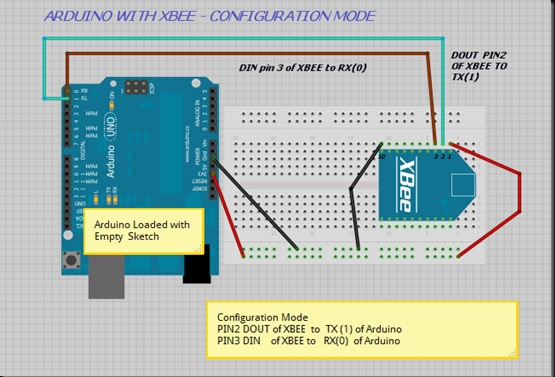
\includegraphics[scale=0.85]{config.jpg}}\par}
\caption{XBEE Connection In Configuration Mode}
\end{figure}

\begin{figure}[h!]
{\centering {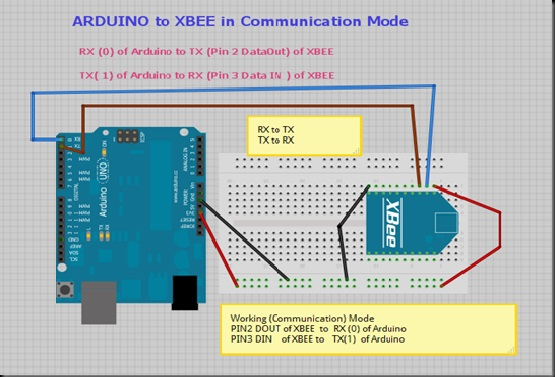
\includegraphics[scale=0.85]{comm.jpg}}\par}
\caption{XBEE Connection In Communication Mode}
\end{figure}
\newpage

\section{Transmitter Code}
int Finger1 = 0;\\
int Finger2 = 1;\\
int Finger3 = 2;\\
int Finger4 = 3;\\
int Finger5 = 4;\\
\\
void setup()\\
{\\
Serial.begin(9600);\\
}\\
\\
void loop()\\
{\\
byte servoValue1;\\
byte servoValue2;\\
byte servoValue3;\\
byte servoValue4;\\
byte servoValue5;\\
\\
int FingerV1 = analogRead(Finger1);\\
int FingerV2 = analogRead(Finger2);\\
int FingerV3 = analogRead(Finger3);\\
int FingerV4 = analogRead(Finger4);\\
int FingerV5 = analogRead(Finger5);\\
\\
if (FingerV1 \textless 200) FingerV1 = 200;\\
else if (FingerV1 \textgreater 460) FingerV1 = 460;\\
if (FingerV2 \textless 200) FingerV2 = 200;\\
else if (FingerV2 \textgreater 460) FingerV2 = 460;\\
if (FingerV3 \textless 200) FingerV3 = 200;\\
else if (FingerV3 \textgreater 460) FingerV3 = 460;\\ 
if (FingerV4 \textless 200) FingerV4 = 200;\\
else if (FingerV4 \textgreater 460) FingerV4 = 460;\\
if (FingerV5 \textless 200) FingerV5 = 200;\\
else if (FingerV5 \textgreater 460) FingerV5 = 460;\\
\\
byte servoVal1 = map(FingerV1,460, 200, 255, 0);\\
byte servoVal2 = map(FingerV2,460, 200, 255, 0);\\
byte servoVal3 = map(FingerV3,460, 200, 255, 0);\\
byte servoVal4 = map(FingerV4,460, 200, 255, 0);\\
byte servoVal5 = map(FingerV5,460, 200, 255, 0);\\
\\
Serial.print(servoVal1);\\
Serial.print(servoVal2);\\
Serial.print(servoVal3);\\
Serial.print(servoVal4);\\
Serial.print(servoVal5);\\
\\
delay(100);\\
}\\
\section{Receiver Code}
#include\\
\\
Servo myservo1; // create servo object to control a servo\\
Servo myservo2;\\
Servo myservo3;\\
Servo myservo4;\\
Servo myservo5;\\
\\
void setup()\\
{\\
Serial.begin(9600);\\
\\
myservo1.attach(2); // attaches the servo on pin 9 to the servo object\\
myservo2.attach(3);\\
myservo3.attach(4);\\
myservo4.attach(5);\\
myservo5.attach(6);\\
}\\
\\
void loop()\\
{\\
if(Serial.available() \textgreater=5)\\
{\\
byte servoAng1 = Serial.read();\\
byte servoAng2 = Serial.read();\\
byte servoAng3 = Serial.read();\\
byte servoAng4 = Serial.read();\\
byte servoAng5 = Serial.read();\\
\\
myservo1.write(servoAng1);\\
myservo2.write(servoAng2);\\
myservo3.write(servoAng3);\\
myservo4.write(servoAng4);\\
myservo5.write(servoAng5);\\
}\\
}\\


\chapter{FUTURE SCOPE}

We Wish to implement and improve the miniproject in the following ways.The XBEE Modules which provides a range limitation for our work need to b replaced with internet protocols,so that surgeries could b done from remote places via internet.The thought of development of a complete Biomorphic Robot can be put into effect.Efforts to implement this system for the development of fireforce rescue missons and military applications.To avoid the misuse of the technology security features like voice command recognition can also implemented.
 

%%%%%%%%%% BIBLIOGRAPHY %%%%%%%%%%
\chapter{Bibliography}
%
\begin{description}

\begin{itemize}

\item www.arduino.cc
\item www.youtube.com
\item alselectro.wordpress.com
\item www.fritzing.org
\item www.sparkfun.com
\item www.nex-robotics.com
\item www.atmel.com

\item O'Reilly Arduino cook book  - Micheal Margolis

\item open software , fashionalable prototyping and wearable computing - samson wiklund,tony olsson

\item Microcontrollers made easy - serge wrolawski

\end{itemize}

\item 

\end{description}

\end{document}
